\section{Motivating Example}

\begin{figure}[htbp]
	\centering
	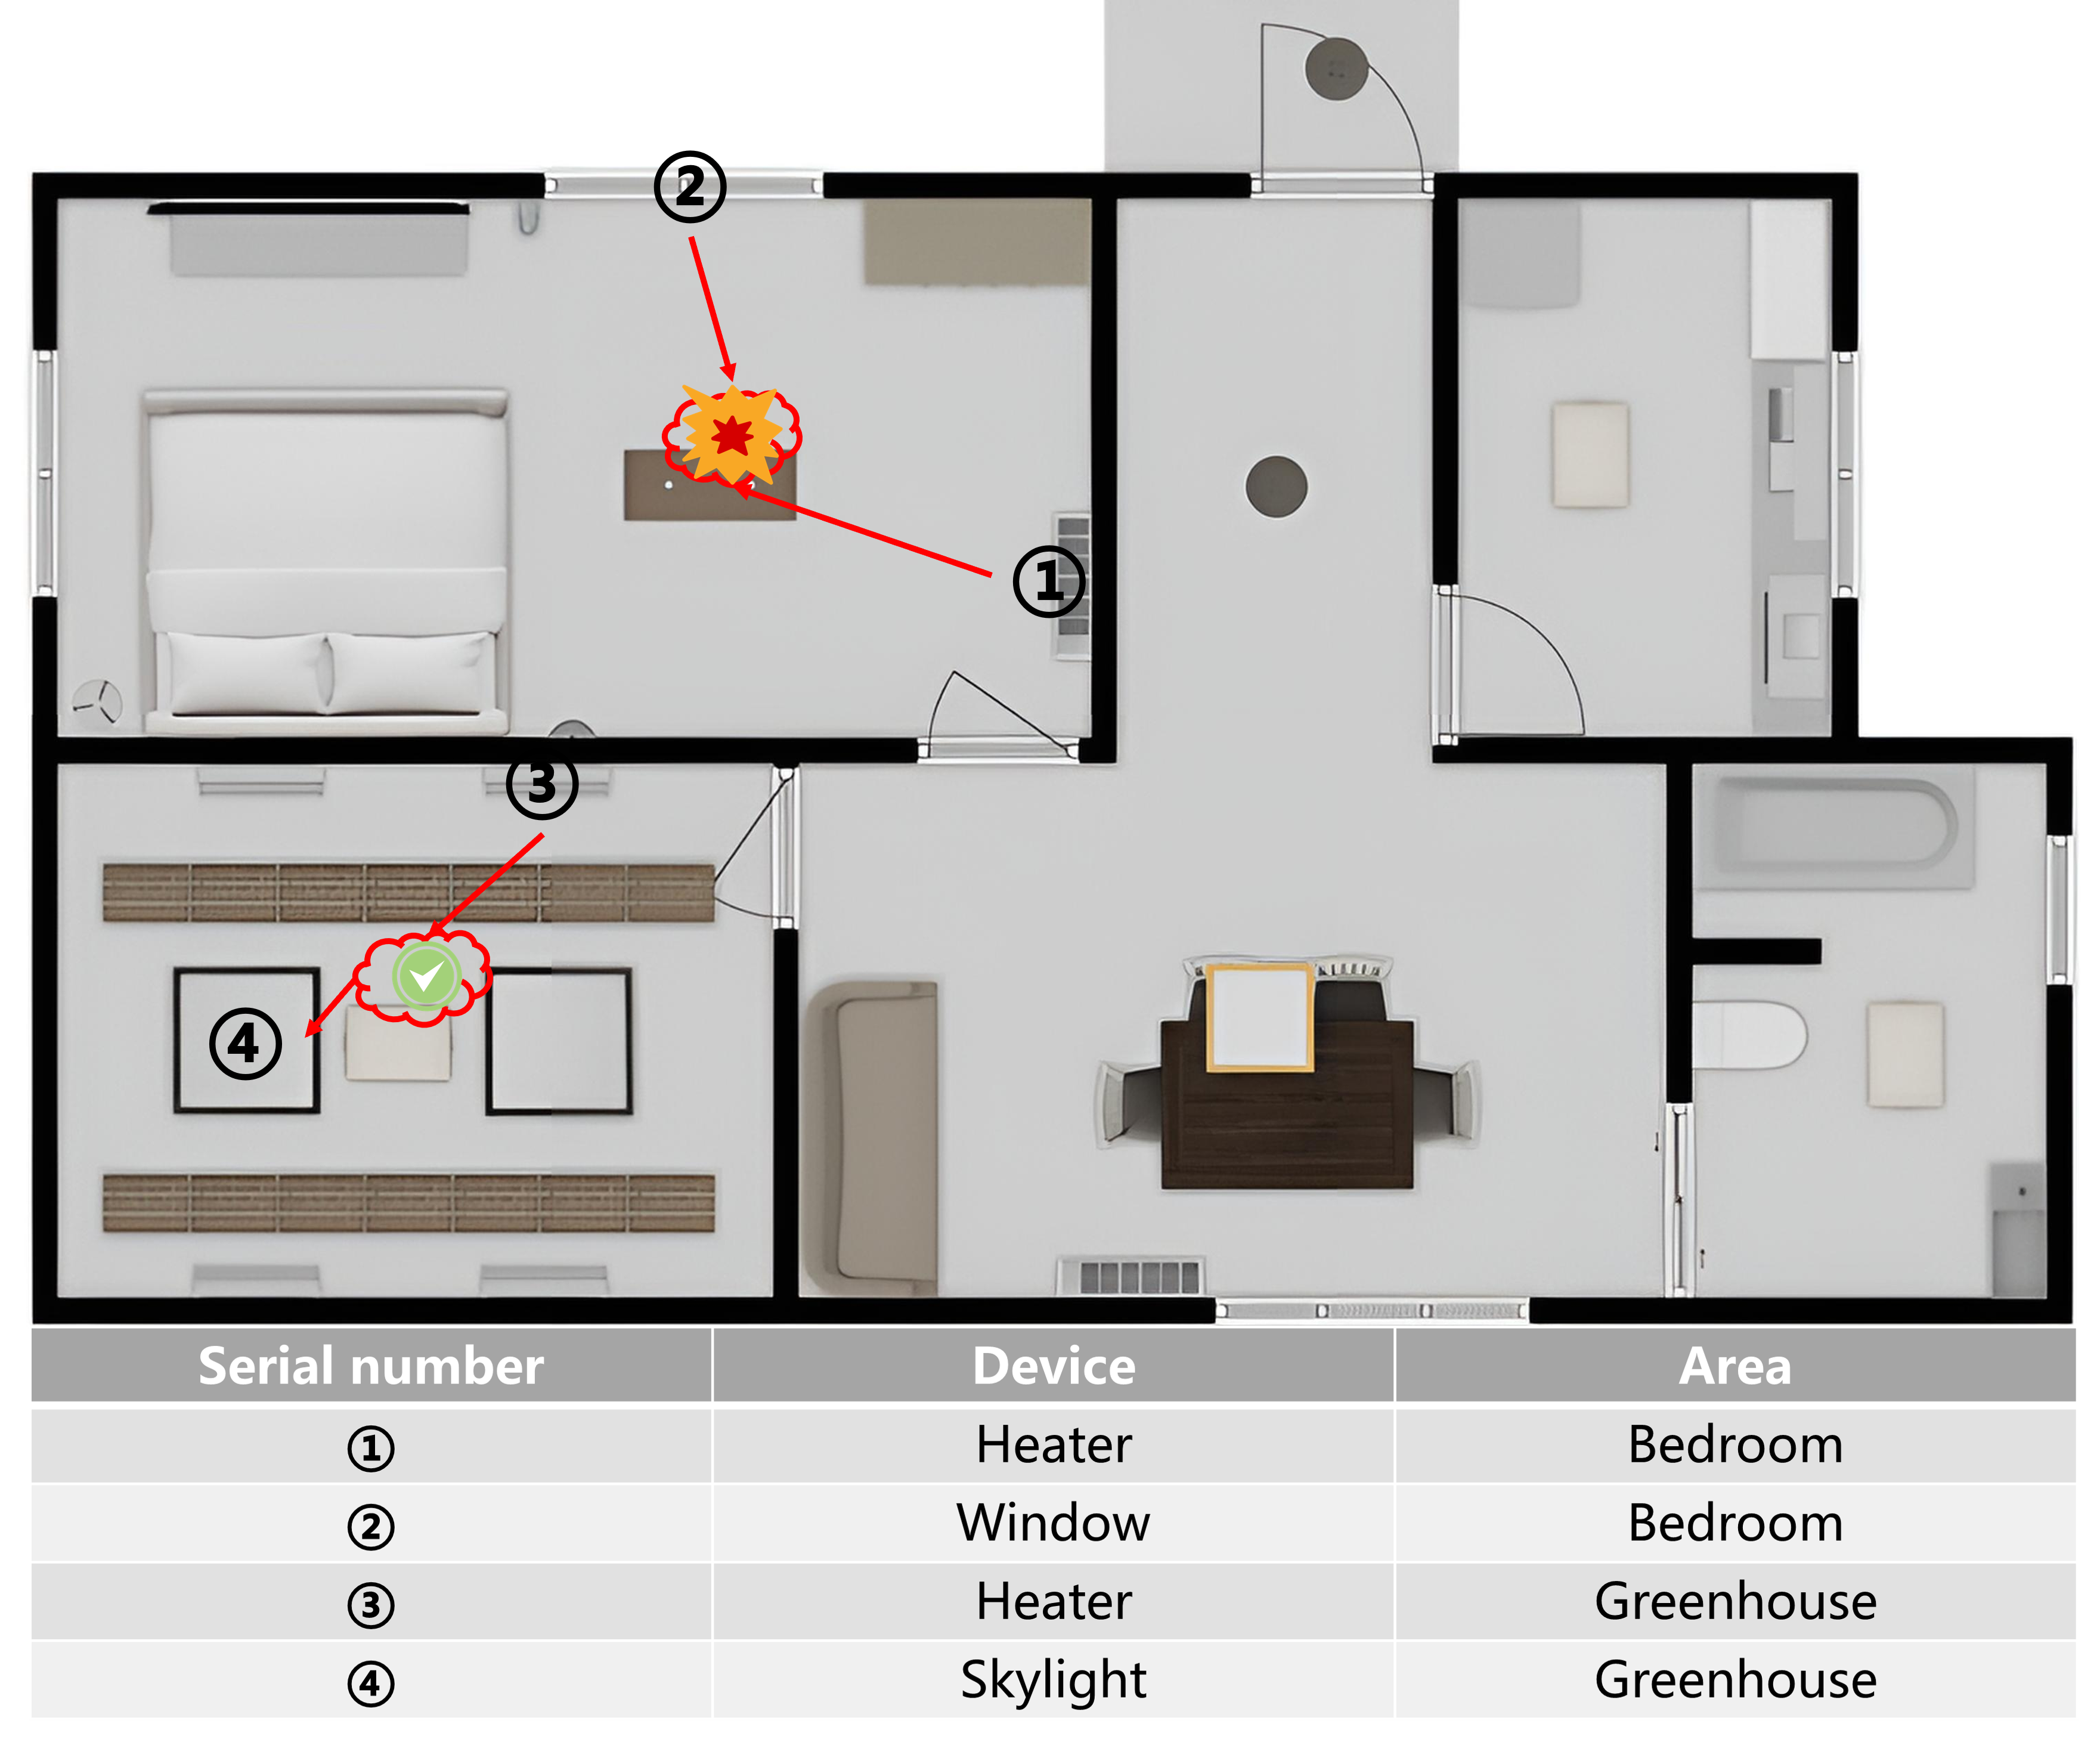
\includegraphics[width=0.4\textwidth]{figure/motivated_example.png}
	\caption{Motivating Example}
	\label{motivated_example}
\end{figure}

% 本节提供了一个具体的例子,以说明规则冲突的特征,并分析现有冲突检测和缓解方法的局限性。图\ref{motivated_example}显示了一个智能家居平面图,包括七个区域:室外(顶部中心)、门廊(中心)、客厅(底部中心)、厨房(右下)、浴室(右下)、卧室(左中)和温室(左下)。其中的\circled{1}是加热器,\circled{2}是卧室窗户,\circled{3}是加热器,\circled{4}是greenhouse的天窗。
This section provides a concrete example to illustrate the characteristics of rule conflicts and analyze the limitations of existing conflict detection and mitigation methods. Figure \ref{motivated_example} shows a smart home floor plan including seven zones: outdoor (top center), porch (center), living room (bottom center), kitchen (bottom right), bathroom (bottom right), bedroom (left center), and greenhouse (bottom left). \circled{1} is a heater, \circled{2} is a bedroom window, \circled{3} is a heater, and \circled{4} is a greenhouse skylight.

% 考虑在温室中设置以下两条规则:规则 1 (R1):当检测到日落时 (触发器),开启加热器 (动作);规则 2 (R2): 当温度达到 30 摄氏度时 (触发器),打开窗户并关闭加热器 (动作)。如图 \ref{motivated_example} 左下角所示,日落时,规则 R1 自动执行,为温室供暖。随着温度持续升高,可能超过 30 摄氏度,触发规则 R2 的执行,导致窗户打开且加热器关闭。在温室中,这种规则交互通常符合用户预期,且不会造成安全问题。然而,若将这两条规则应用于卧室,情况则截然不同。规则 R1 通过提高卧室温度触发规则 R2,进而打开窗户。卧室的窗户通常不是自动天窗,且在用户不知情的情况下打开窗户会带来安全隐患。攻击者甚至可能利用这些规则,创建恶意执行路径,从而控制窗户、门锁等安全敏感设备。
	Consider the following two rules set in the greenhouse: Rule 1 (R1): When sunset is detected (trigger), turn on the heater (action); Rule 2 (R2): When the temperature reaches 30\celsius (trigger), open the window and turn off the heater (action). As shown in the bottom left corner of Fig. \ref{motivated_example}, at sunset, rule R1 is automatically executed, providing heat to the greenhouse. As the temperature continues to rise, it may exceed 30\celsius, triggering the execution of rule R2, which causes the window to open and the heater to turn off. In a greenhouse, this rule interaction is usually in line with user expectations and does not cause security problems. However, if these two rules are applied to the bedroom, the situation is very different. Rule R1 triggers the execution of rule R2 by raising the bedroom temperature, which in turn opens the windows. Bedroom windows are usually not automatic skylights, and opening the windows without the user's knowledge can create security risks. Attackers may even exploit these rules to create malicious execution paths to control security-sensitive devices such as windows and door locks.

% 上述示例揭示了规则交互的复杂性。规则间的相互影响并非仅限于直接作用 (例如,两条同时执行的规则,一条设置为制热模式,另一条设置为制冷模式),也可能通过温度、湿度、亮度、声音等间接途径产生。因此,在检测规则冲突时,必须考虑来自其他渠道的潜在冲突。此外,规则冲突具有地域性和用户主观性。相同的规则交互在温室中可能被认为是正常行为,而在卧室中则可能被视为冲突。用户主观性体现在对同一组规则交互的不同解读:一些用户可能认为卧室空调的除湿模式和加湿器交替工作是为了维持空气湿度,属于正常交互,而另一些用户则可能认为这是一种资源浪费。再者,智能家居系统中对侧面通道的检测不应仅限于温度、湿度等参数,还应具备地域属性。例如,门廊的灯光可能影响厨房和客厅的亮度,但通常不会影响卧室。因此,同时执行的两条与亮度相关的规则可能不会实际发生交互。
The above example reveals the complexity of rule interactions. The interaction between rules is not limited to direct effects (e.g., two rules executing simultaneously, one set to heating mode and the other to cooling mode), but can also be generated through indirect channels such as temperature, humidity, brightness, and sound. Therefore, when detecting rule conflicts, it is necessary to consider potential conflicts from other channels. In addition, rule conflicts have regionality and user subjectivity. The same rule interaction may be considered normal behavior in a greenhouse, but may be considered a conflict in a bedroom. User subjectivity is reflected in different interpretations of the same set of rule interactions: Some users may consider the alternating operation of the dehumidification mode and the humidifier in the bedroom to maintain air humidity as a normal interaction, while others may consider it a waste of resources. Furthermore, the detection of side channels in smart home systems should not be limited to parameters such as temperature and humidity, but should also have regional attributes. For example, porch lights may affect the brightness of the kitchen and living room, but usually do not affect the bedroom. Therefore, two brightness-related rules executed at the same time may not actually interact.

% 若采用基于安全策略的方法进行冲突检测,用户需投入大量精力,因为不同家庭的户型、设备配置等差异会导致安全策略的定制需求各不相同。这不仅需要专业人员的参与,而且定制的安全策略很可能无法涵盖所有可能的冲突场景。另一方面,若仅根据规则交互模式进行判断,虽然能检测到卧室中发生的冲突,但也会将温室中的规则交互误判为冲突。随着规则数量的增加,误报数量会急剧上升,用户需要逐一核实,从而显著增加用户负担。
If a security policy-based approach is used for conflict detection, users need to invest a lot of effort, because the customization needs of security policies will vary from home to home due to differences in housing types, equipment configurations, etc. This not only requires the participation of professionals, but the customized security policies are likely to fail to cover all possible conflict scenarios. On the other hand, if the judgment is based solely on the rule interaction mode, the conflicts occurring in the bedroom can be detected, but the rule interaction in the greenhouse will be misjudged as a conflict. As the number of rules increases, the number of false positives will increase sharply, and users need to verify them one by one, thus significantly increasing the user burden.

% 若采取更改规则配置的方法,可能会避免规则冲突,但是更多的情况是无法实现用户期望的自动化功能,甚至引入其他规则冲突。若采取基于安全策略的方法避免规则冲突,在当前智能家居系统中比较容易实现,但是该方法很难推广到环境各异的不同用户家庭。
If the method of changing rule configurations is adopted, rule conflicts may be avoided, but in most cases, the expected automation functions cannot be achieved, and even other rule conflicts may be introduced. If the method based on security policies is adopted to avoid rule conflicts, it is relatively easy to implement in the current smart home system, but this method is difficult to promote to different users' home with different environments.

% 由此我们总结出以下挑战。
According to above motivating example, we summarize the following challenges.

%智能家居系统中规则冲突的定义没有统一定义。一对规则的交互是否属于规则冲突存在模糊定义,\ref{huang2023survey}基于对相关工作的调研认为,多个物联网规则可能共存于共享的家庭环境中,并同时运行,同时执行多个物联网规则可能会导致意想不到的后果,即使每个物联网规则都是独立正确的,该现象被称为规则冲突。“意想不到的后果”除了包括明确的对安全存在明显威胁的运行结果,还包括用户预期之外且非用户意向的运行结果,则一次规则交互是否是规则冲突取决于用户的主观感受,或者称为个人偏好,如何找到该类型的规则交互是一个挑战。

%用户的家居环境具有多样性。不同用户的智能家居系统具有差异性,家庭中布局、智能家居设备多种多样,特定的安全策略虽然能够有效避免已经发现的规则冲突,但是其泛化能力弱,难以移植到不同家庭环境,且不能覆盖所有规则冲突,不能广泛使用,采用检测规则交互的判定方法容易产生较多误报,从而导致用户工作量较大,设计一个泛化能力强且检测与效果优异的冲突检测处理方案是一个挑战。

%当前规则冲突检测处理方案对用户不友好。规则冲突检测中使用规则交互模式的检测方法存在显著的误报。特定的安全策略针对特定的家庭,相同的安全策略很难推广到不同家庭,且该方法只能用于防止已经发生的规则冲突,它与重新配置规则都具有相同的缺陷:用户工作量大、需要具有相关专业知识的人员指导、难以大范围推广,设计一个用户友好的,有效自动化程度高、便于非专业用户实现的规则冲突检测与处理方案是一个挑战。


\begin{itemize}
	\item \textbf{C1}: The definition of rule conflicts in smart home systems lacks a unified standard. Whether the interaction of a pair of rules constitutes a rule conflict is ambiguously defined. \ref{huang2023survey} suggests that multiple IoT rules may coexist and run simultaneously in a shared home environment. The simultaneous execution of multiple IoT rules may lead to unintended consequences, even if each IoT rule is independently correct. This phenomenon is called a rule conflict. "Unintended consequences" include not only operational results that clearly pose a security threat but also operational results that are unexpected and unintended by the user. Thus, whether a rule interaction is a rule conflict depends on the user's subjective feelings, or personal preferences. Finding this type of rule interaction is a challenge.
	
	\item \textbf{C2}: Users' home environments are diverse. Smart home systems vary among different users, with diverse layouts and smart home devices in households. Although specific security policies can effectively avoid already discovered rule conflicts, their generalization ability is weak, making them difficult to transfer to different home environments and failing to cover all rule conflicts, thus preventing their widespread use. The method of determining rule interaction is prone to generating many false positives, resulting in a large workload for users. Designing a conflict detection and resolution scheme with strong generalization ability and excellent detection effect is a challenge.
	
	\item \textbf{C3}: Current rule conflict detection and resolution schemes are not user-friendly. The rule interaction pattern detection method used in rule conflict detection has significant false positives. Specific security policies are designed for specific homes, and the same security policies are difficult to promote to different homes. Moreover, this method can only be used to prevent rule conflicts that have already occurred. It shares the same drawbacks as reconfiguring rules: high user workload, the need for guidance from professionals with relevant expertise, and difficulty in large-scale promotion. Designing a user-friendly rule conflict detection and resolution scheme that is effective, highly automated, and easy for non-professional users to implement is a challenge.
\end{itemize}

%对于以上列出的挑战,我们使用以下解决方法
For the challenges listed above, we use the following solutions.

%我们采用逐步完善的思路寻找规则冲突,并将用户偏好通过配置文件的形式融入到检测标准中:首先结合用户家庭环境特征对规则进行重新建模,用户只需要根据指导提供与规则相关的区域信息即可快速完成;然后进行形式化分析,检测出所有可能的规则交互;接下来将根据用户提交的实体安全信息,自动化检测出违反实体安全信息的规则交互,视为规则冲突,同时用户可以根据偏好,根据对规则交互的描述选择一堆规则交互是否为规则冲突。

%丰富side channel的概念,包括area、channel与trend三个层面,对规则进行重新建模,从而使得方案适应因为用户家居环境的多样性,且采用用户的安全实体配置而非固定的安全配置进行规则冲突检测。在规则冲突处理方面,针对不同类型的规则冲突,设计了多个处理策略模板,并根据具体的冲突信息进行填充。每个规则冲突都可以获得有针对性的处理策略选项,并根据规则冲突的特点选择相应的处理策略。从而实现优异的泛化能力

%在规则冲突检测的过程中使用用户友好界面,指导用户提供需要的信息,如自动化检测出违反实体安全信息的规则交互被视为规则冲突后,将会展示出详细的冲突信息,用户可以根据个人偏好选择冲突处理策略,用户也可以检查所有的规则交互信息(自然语言格式),并指定规则交互处理策略,避免用户不期望的规则交互发生,所有规则冲突检测与处理均为自动化执行,同时通过用户界面向用户展示优化后的自然语言描述,辅助用户进行相关个人偏好的配置和保留用户最高权限决策的能力。

\begin{itemize}
	\item \textbf{S1}:We adopt a step-by-step refinement approach to identify rule conflicts, and incorporate user preferences into the detection criteria through configuration files. First, we remodel the rules by incorporating the characteristics of the user's home environment. Users only need to provide region information related to the rules according to the guidance to quickly complete the setup. Then, we perform formal analysis to detect all possible rule interactions. Next, based on the entity security information submitted by the user, we automatically detect rule interactions that violate entity security information, which are considered rule conflicts. Simultaneously, users can choose whether a pair of rule interactions constitutes a rule conflict based on their preferences and the description of the rule interaction.
	
	\item \textbf{S2}: We enrich the concept of side channels, including the three levels of area, channel, and trend, and remodel the rules, so that the scheme adapts to the diversity of users' home environments. We also use the user's security entity configuration instead of a fixed security configuration for rule conflict detection. In terms of rule conflict resolution, we have designed multiple processing strategy templates for different types of rule conflicts and fill them in according to specific conflict information. Each rule conflict can obtain targeted processing strategy options, and the corresponding processing strategy is selected according to the characteristics of the rule conflict. This achieves excellent generalization ability.
	
	\item \textbf{S3}: In the rule conflict detection process, a user-friendly interface is used to guide users in providing the necessary information. For example, after automatically detecting rule interactions that violate entity security information as rule conflicts, detailed conflict information will be displayed. Users can choose conflict resolution strategies according to their personal preferences. Users can also check all rule interaction information (in natural language format) and specify rule interaction resolution strategies to avoid unwanted rule interactions. All rule conflict detection and resolution are executed automatically, while the optimized natural language description is displayed to the user through the user interface, assisting the user in configuring related personal preferences and retaining the ability for the user to make the highest-level decisions.
\end{itemize}